
%%%%%%%%%%%%%%%%%%%%%%%%%%%%%%%%%%%%%%%%%%%%%%%%%%%%%%%%%%%%%%%%%%%%%%%%%%%%%%%%
%%%%%%%%%%%%%%%%%%%%%%%%%%%%%%%%%%%%%%%%%%%%%%%%%%%%%%%%%%%%%%%%%%%%%%%%%%%%%%%%
\section{\textcolor{blue}{ Treino dividir  a atenção}}


Tabela \ref{fig:treino-bolinha1}.

Pausando no meio da música para voltar a pegar o tempo forte.

\begin{table}[!h]
  \centering
    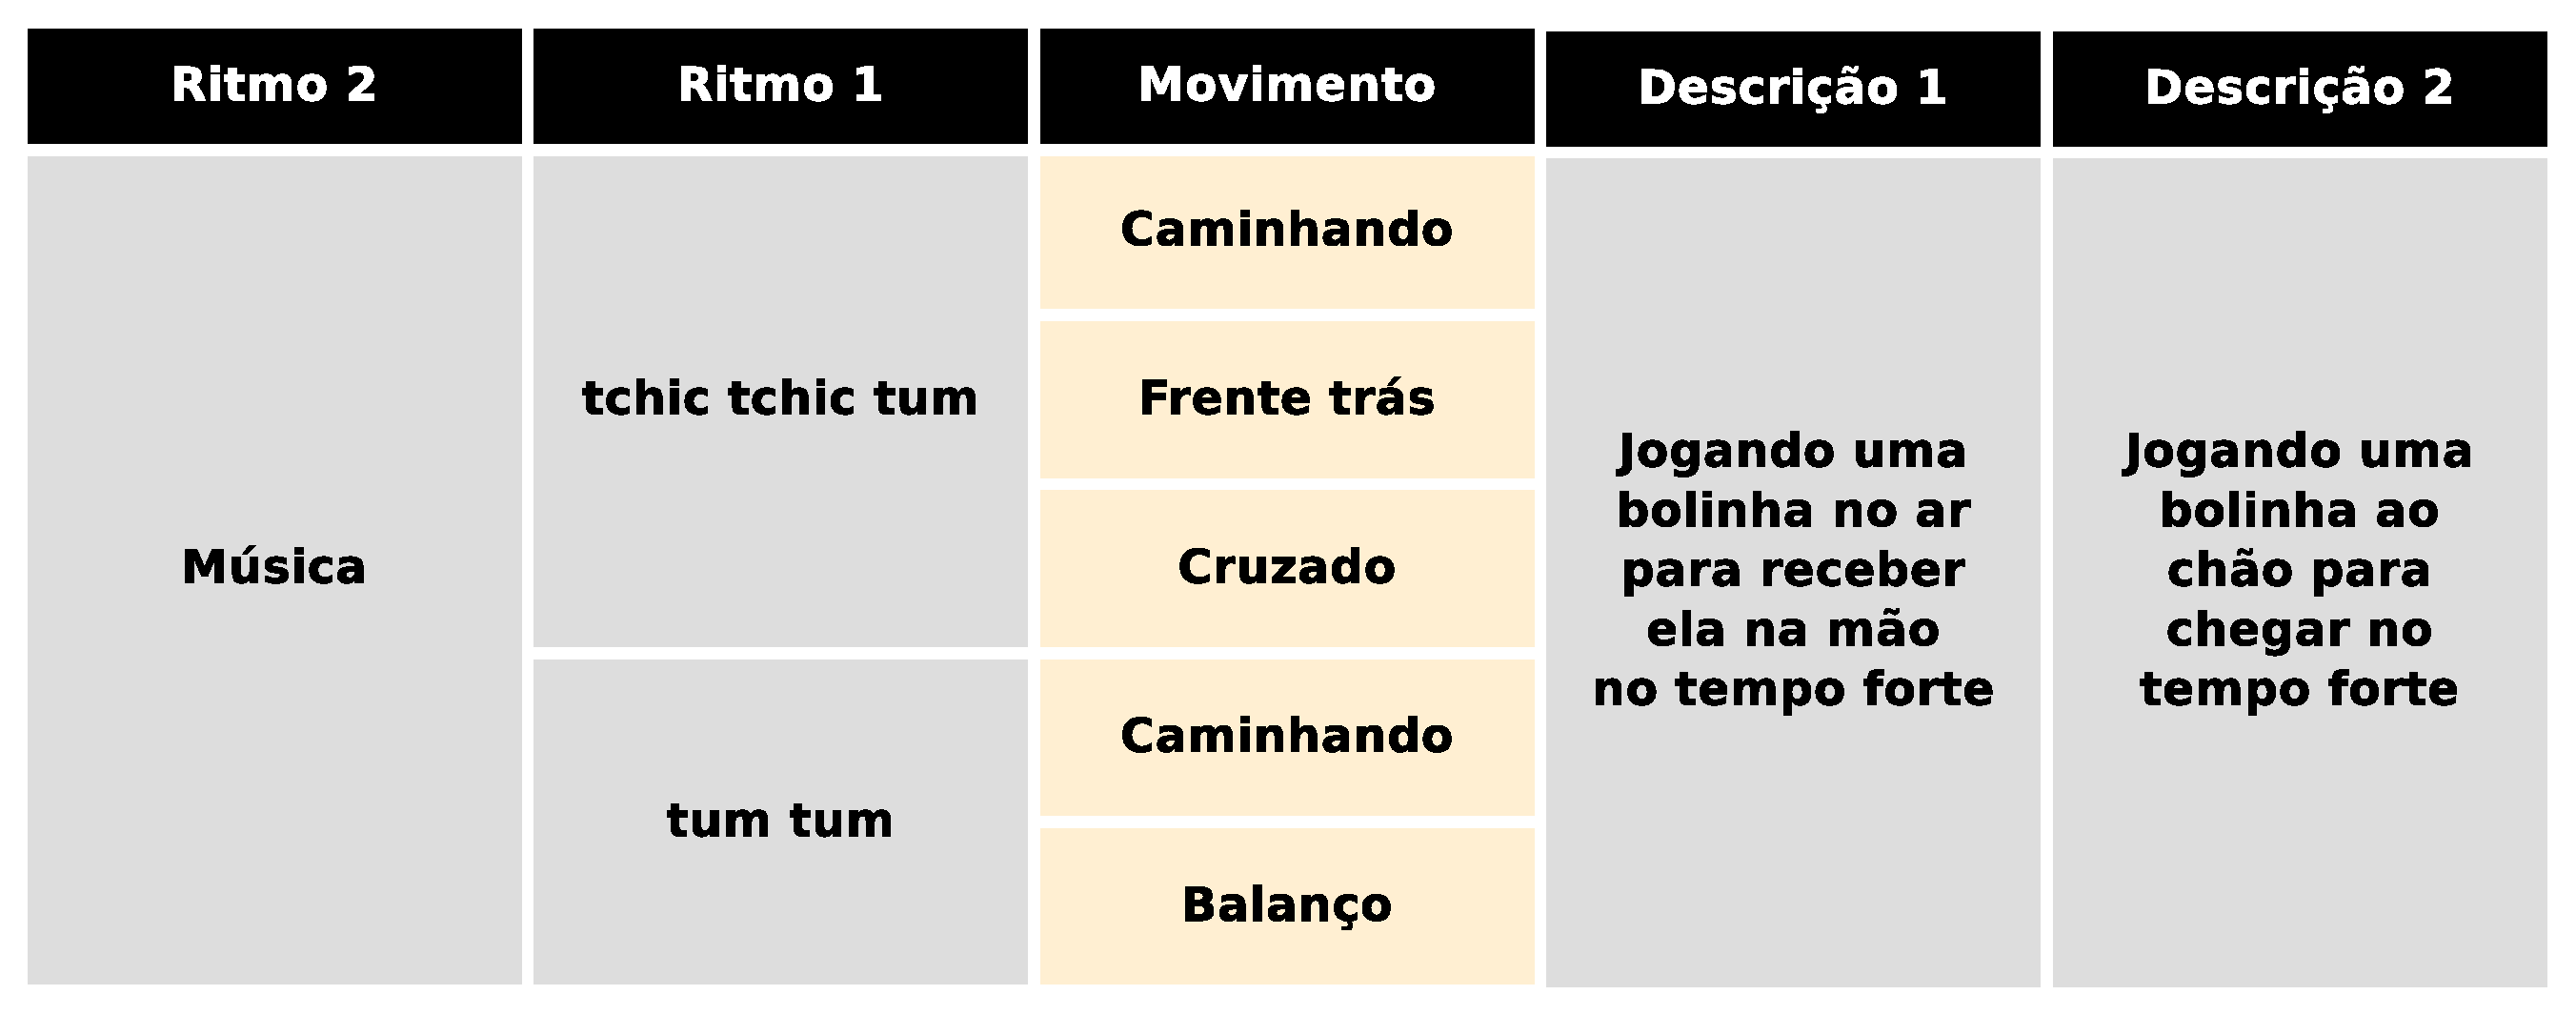
\includegraphics[width=1.0\textwidth]{chapters/cap-body-control/treino-bolinha1.eps}
\caption{Treinamentos simples.}
\label{fig:treino-bolinha1}
\end{table}

Figura \ref{fig:treino-bolinha2}.

\begin{table}[!h]
  \centering
    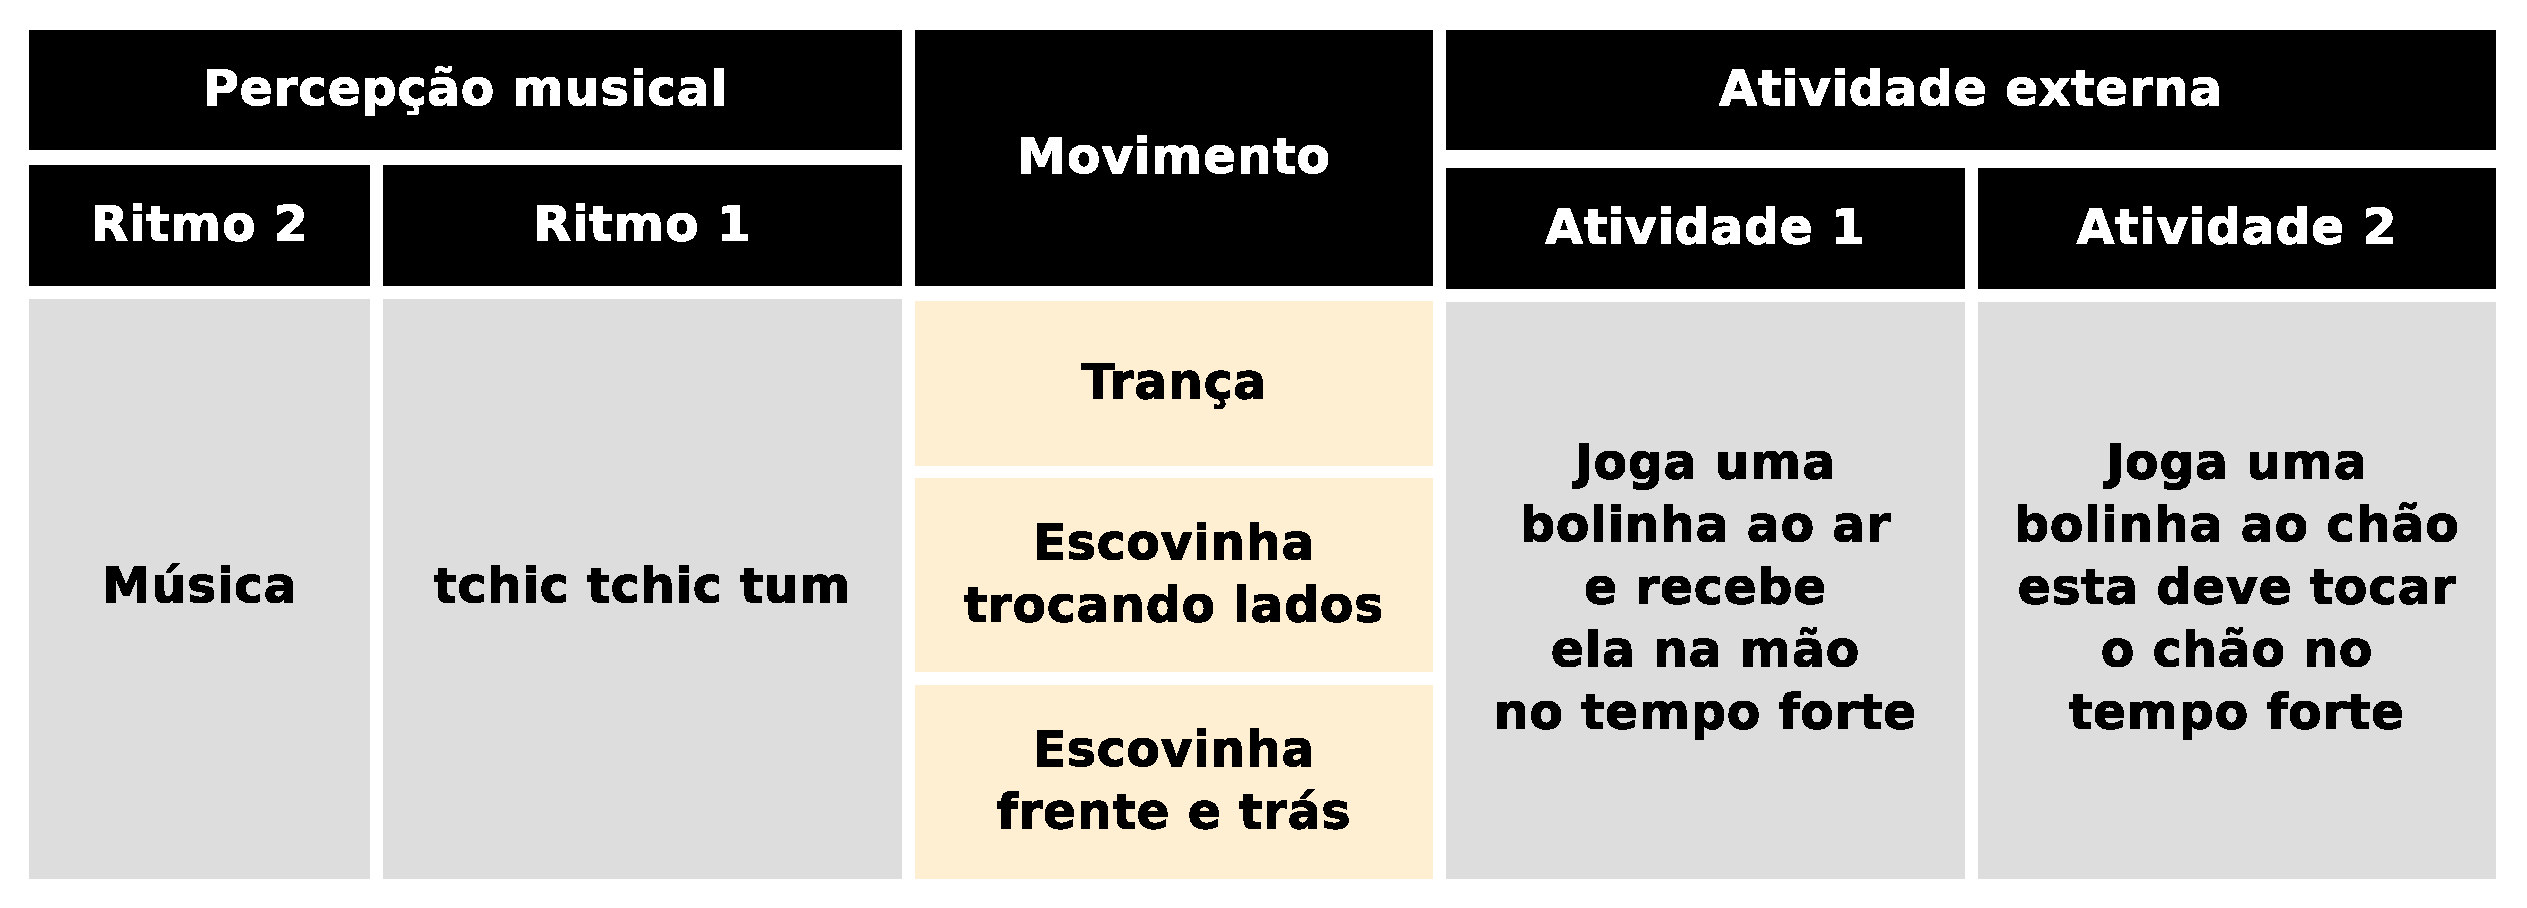
\includegraphics[width=1.0\textwidth]{chapters/cap-body-control/treino-bolinha2.eps}
\caption{Treinamentos complexos.}
\label{fig:treino-bolinha2}
\end{table}

Figura \ref{fig:treino-bolinha3}.

\begin{table}[!h]
  \centering
    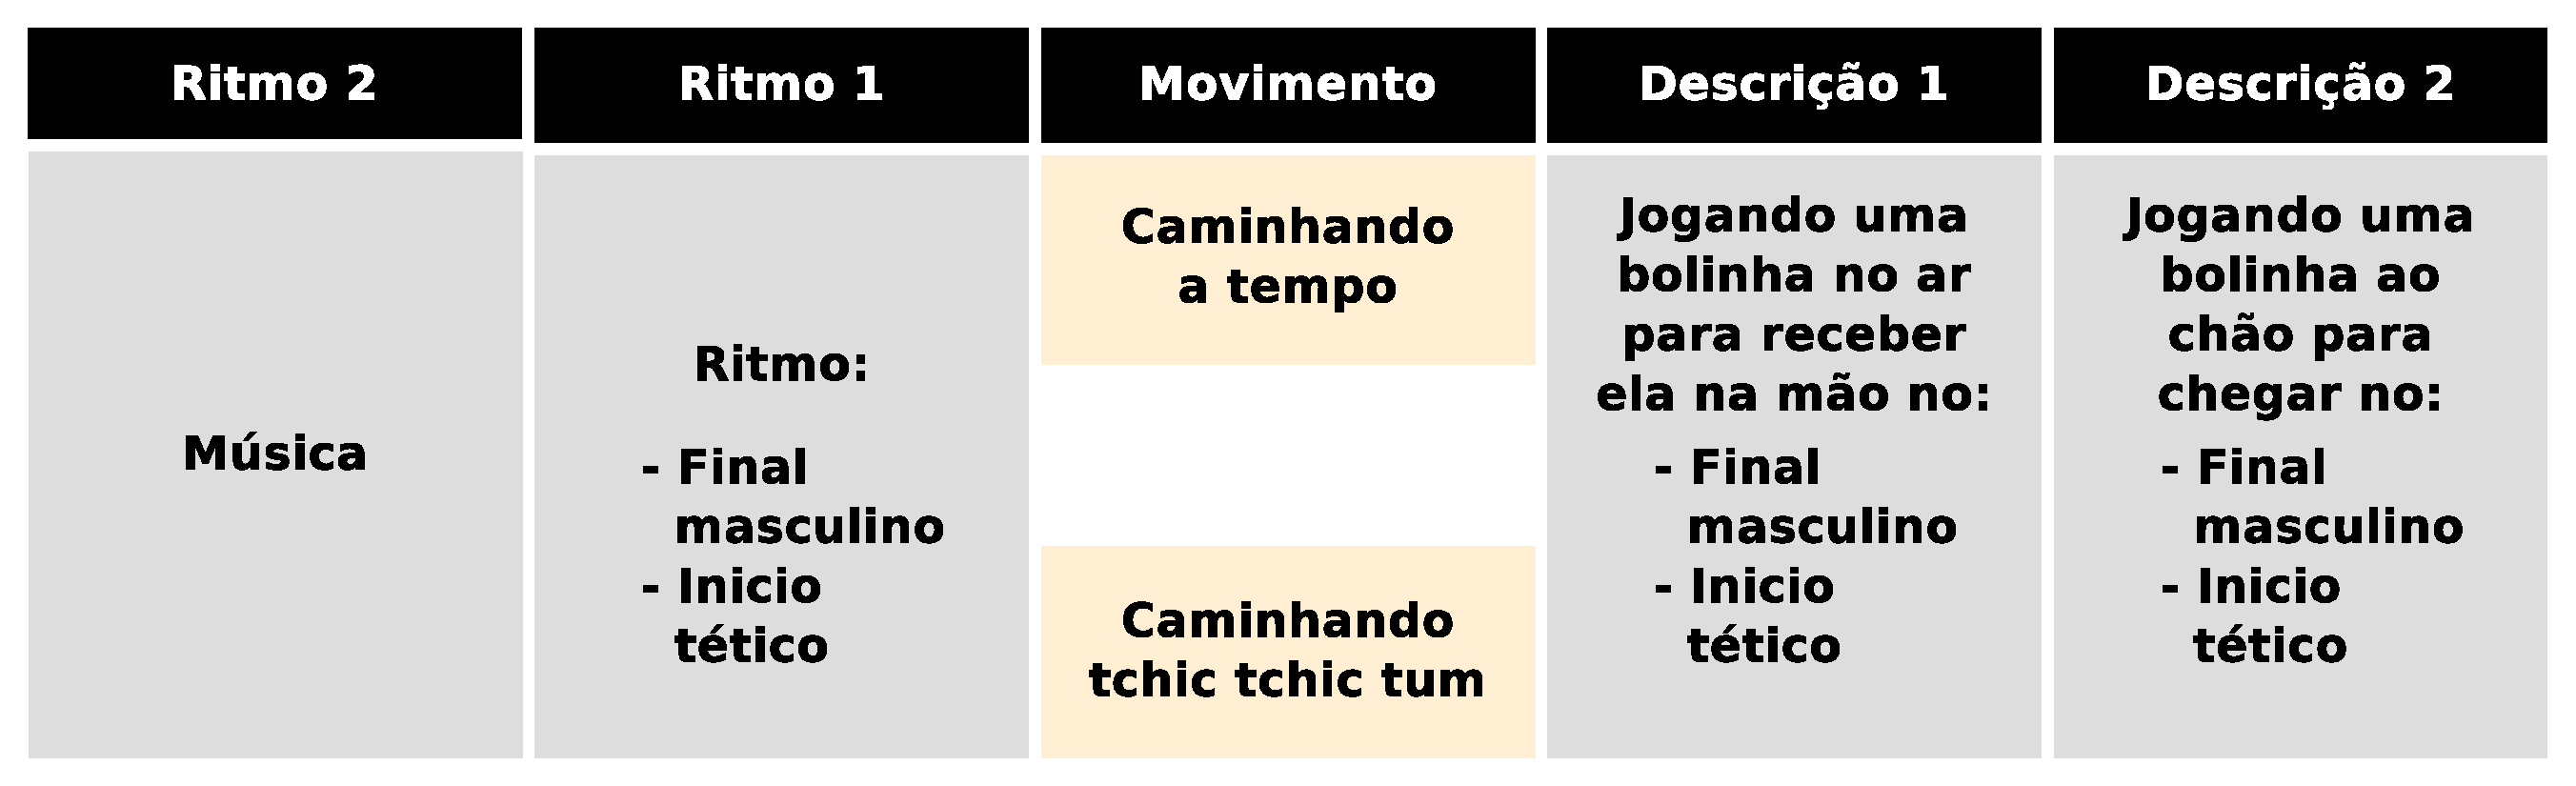
\includegraphics[width=1.0\textwidth]{chapters/cap-body-control/treino-bolinha3.eps}
\caption{Treinamentos simples.}
\label{fig:treino-bolinha3}
\end{table}

Figura \ref{fig:treino-bolinha4}.

\begin{table}[!h]
  \centering
    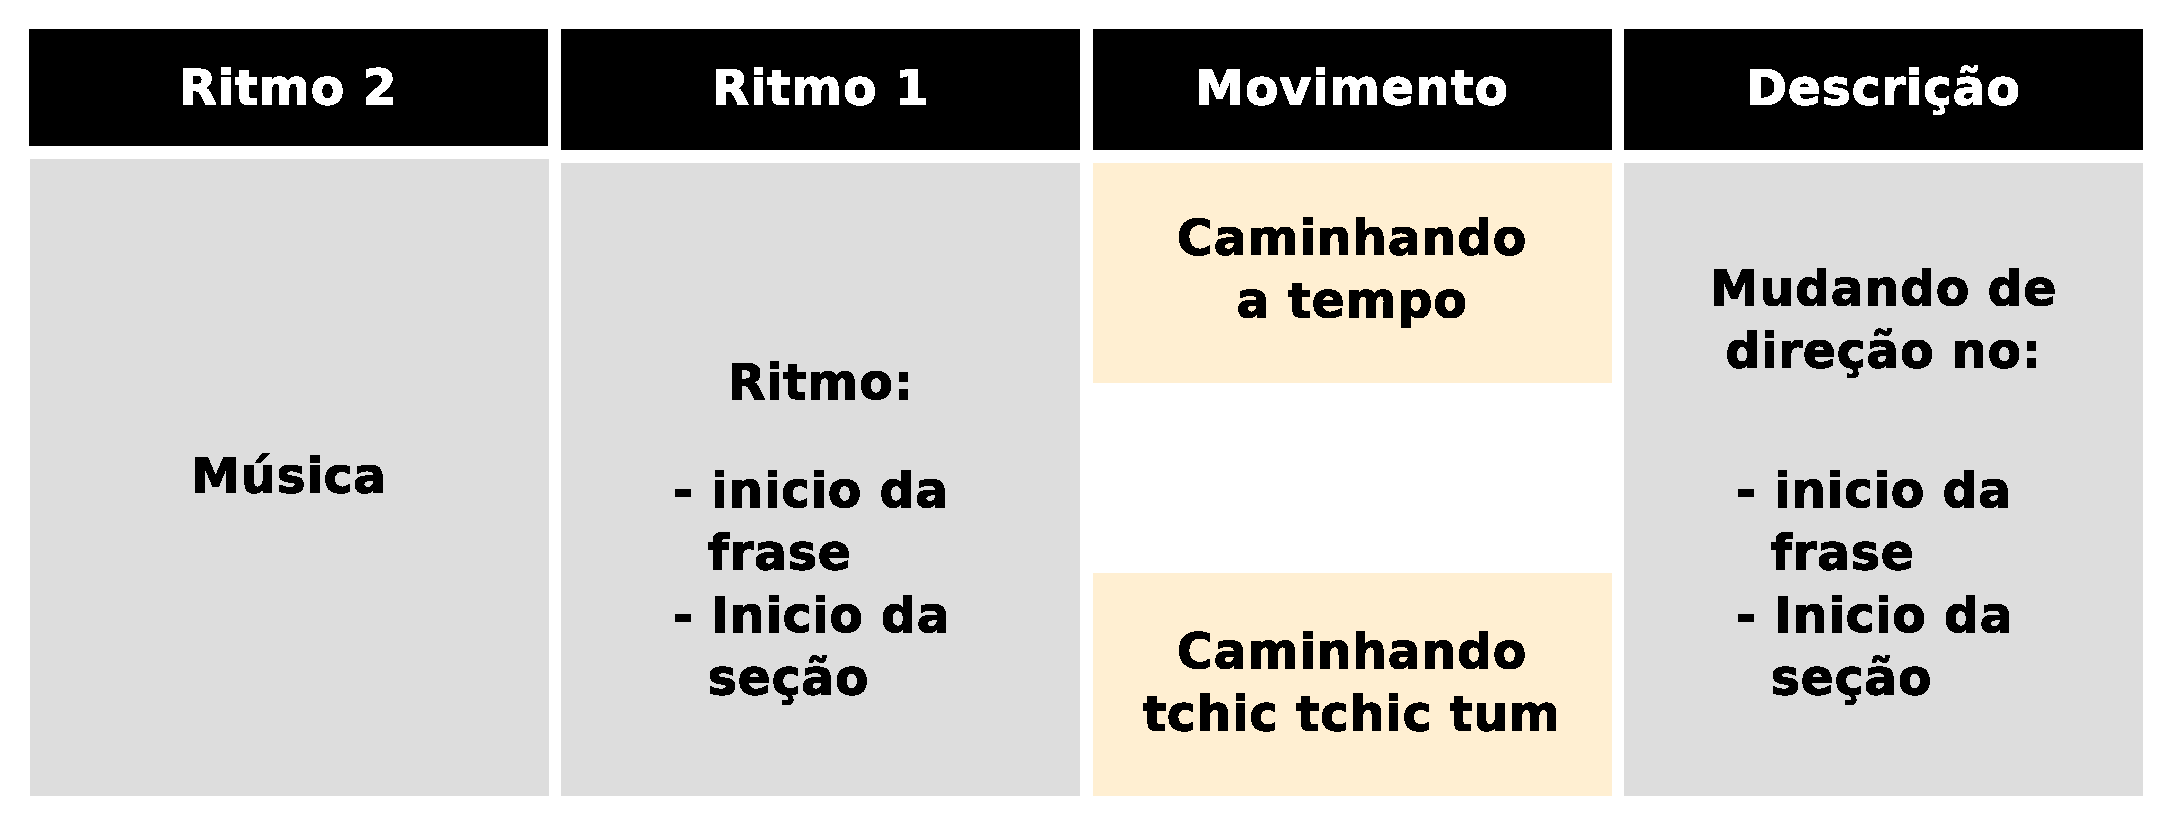
\includegraphics[width=0.75\textwidth]{chapters/cap-body-control/treino-bolinha4.eps}
\caption{Treinamentos seguindo frases.}
\label{fig:treino-bolinha4}
\end{table}

%%%%%%%%%%%%%%%%%%%%%%%%%%%%%%%%%%%%%%%%%%%%%%%%%%%%%%%%%%%%%%%%%%%%%%%%%%%%%%%%
%%%%%%%%%%%%%%%%%%%%%%%%%%%%%%%%%%%%%%%%%%%%%%%%%%%%%%%%%%%%%%%%%%%%%%%%%%%%%%%%
\section{\textcolor{blue}{ Treino de ombros e quadril no plano frontal}}

Figura \ref{fig:pessoalombroquadril1}.

\begin{figure}[!h]
  \centering
    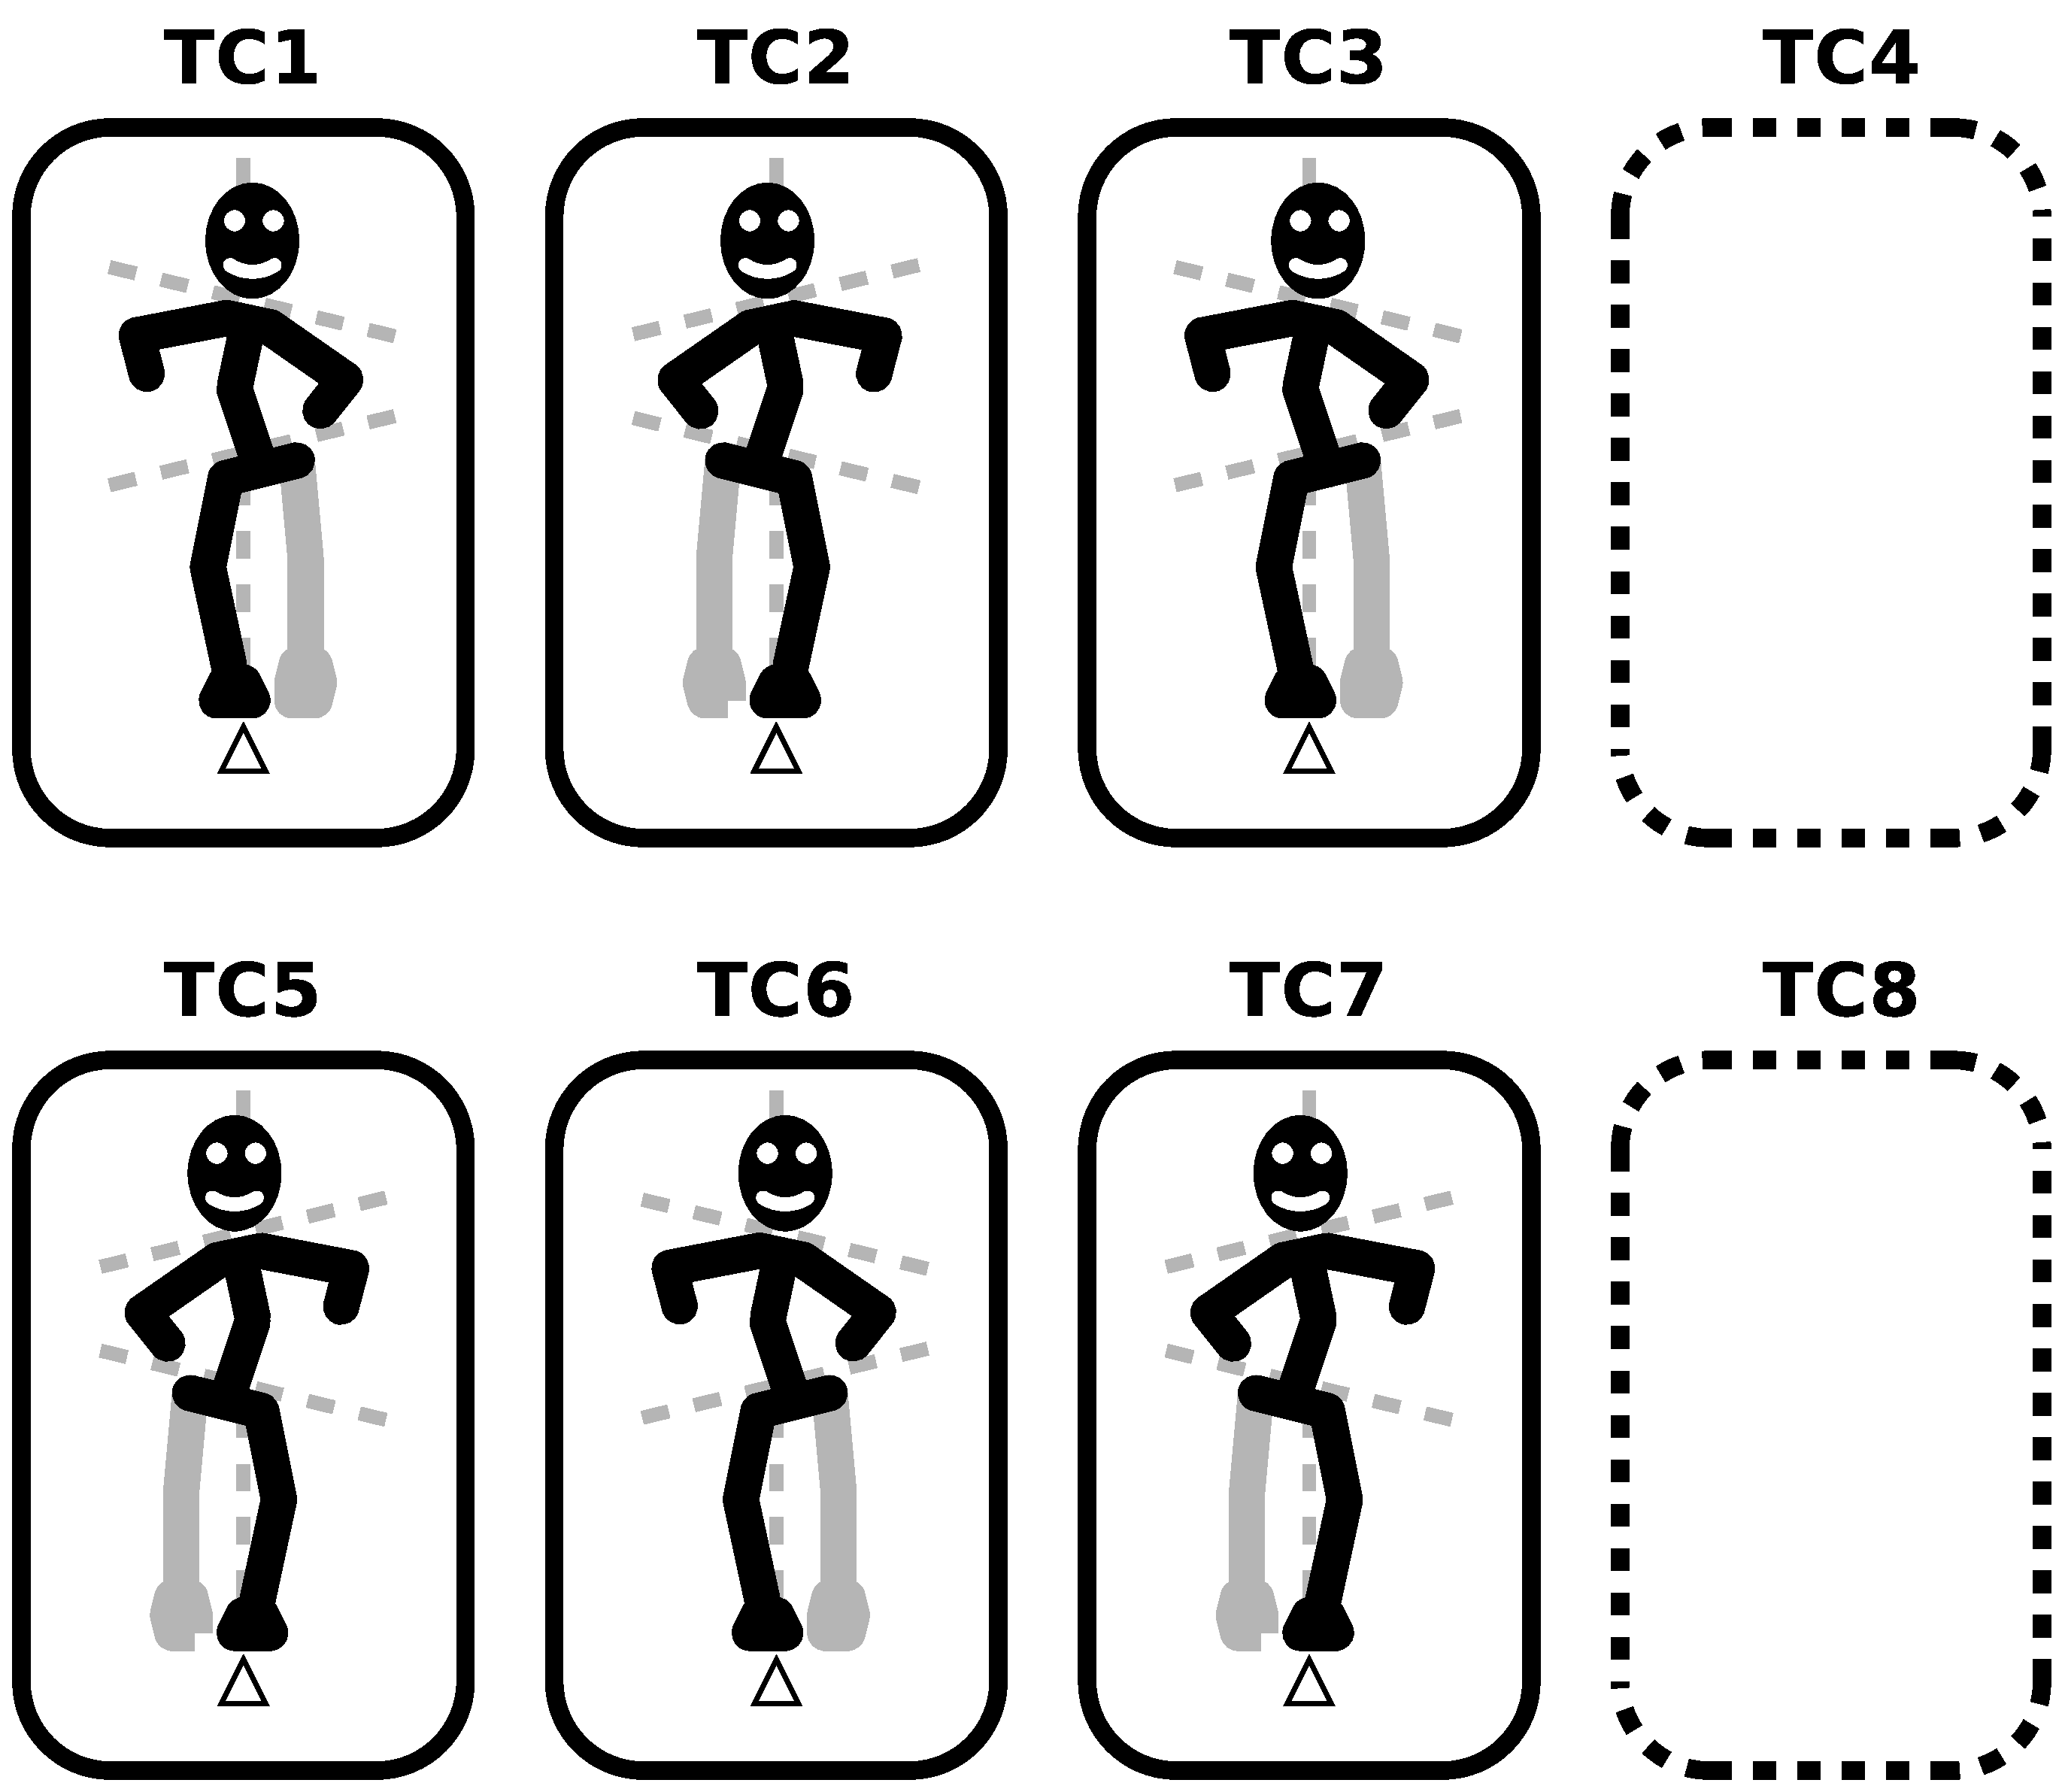
\includegraphics[width=\textwidth]{chapters/cap-body-control/postura-ombro1.eps}
\caption{Diagrama de tempos coreográficos para o treino ombros e quadril, $T=2~TC$.}
\label{fig:pessoalombroquadril1}
\end{figure}

\section{\textcolor{red}{  Treino de ombros no plano frontal}}

\section{\textcolor{red}{  Treino do quadril no plano frontal}}

